\documentclass{article}
\usepackage{amsmath, amssymb,amsthm}
\usepackage{graphicx}

\begin{document}

\section*{Ruína do Jogador}

Considere um jogador que com capital \( x \in (-B, A) \) a cada passo 
\begin{itemize}
\item ganha R\$1 com probabilidade \( \tfrac{1}{2} \) (vai para \( x+1 \)), ou
\item perde R\$1 com probabilidade \( \tfrac{1}{2} \) (vai para \( x-1 \)),
\end{itemize}
de modo independente.  

O processo termina quando o jogador ganha $A$  (vitória) ou perde $B$ (falência).

Se o capital inicial é $S_0$ então após $n$ rodadas
$$
S_n =S_0 + X_1+\cdots+X_n
$$
onde $X_i$ é uma variável aleatória que assume valore em $\{-1,+1\}$
com probabilidade $\tfrac 12$, ela representada o resultado de cada
rodada. Uma vez que $S_n = S_0+A$ ou $S_n=S_0 -B$ o processo
$X_1,X_2,X_3,\dots$ fica com o valor fixo atingido.

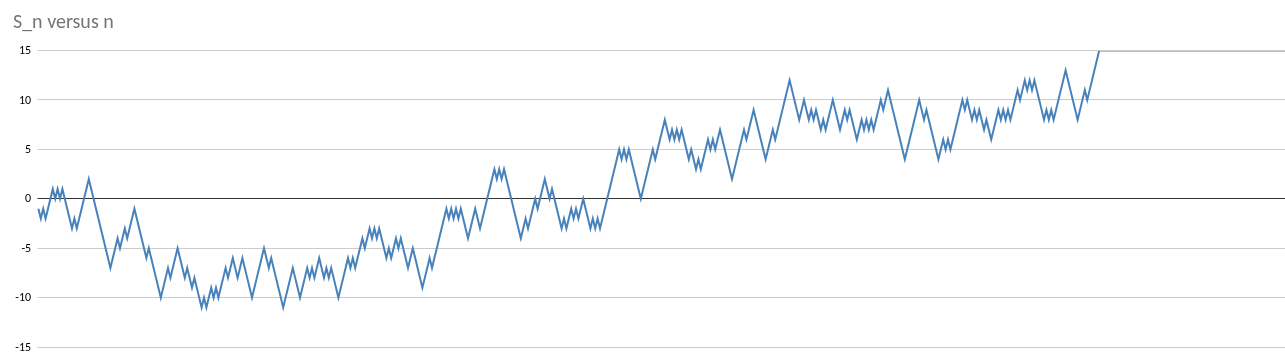
\includegraphics[width=\textwidth]{srw.png}


A variável
aleatória
$$
\tau= \min\{n\geq \colon S_n = S_0+A \text{  ou } S_n=S_0 -B\}
$$
é chamada \textbf{tempo de parada}.

Note que podemos assumir que $S_0=0$.

\subsection*{1. Probabilidade de vitória}

Seja \( p(x) = \mathbb{P} (S_n = A \,|\, S_0=x)\), para $-B<x<A$, a
probabilidade de atingir \( A \) antes de \( -B \), começando com
capital \( x \in (-B,A) \). Então
\[
p(x) =
\displaystyle \frac{x + B}{A + B},  \quad (\forall x,~ -B < x < A)
\]
e $p(x) = 1$ se $x \geq A$  e 
e $p(x) = 0$ se $x \leq -B$.


\begin{proof}[Demonstração]
  Para \( -B < x < A \), depois do primeiro passo o capital do jogador
  ou é $x+1$ como probabilidade $\tfrac 12$ ou o capital é $x-1$ com
  probabilidade $\tfrac 12$. Usamos a lei de probabilidade total e obtemos  a equação de recorrência
  \[
    p(x) = \frac{1}{2}p(x+1) + \frac{1}{2}p(x-1)
  \]
  com condições de contorno dadas por \( p(-B) = 0\) e \(p(A) = 1\).
  De \( p(x) = \frac{1}{2}p(x+1) + \frac{1}{2}p(x-1) \) obtemos
  \begin{align*}
    p(x+1) - p(x) - (p(x) - p(x-1))= 0 &\Leftrightarrow 
    \Delta p(x) - \Delta p(x-1) = 0 \\&\Leftrightarrow
    \Delta^2 p(x) = 0
  \end{align*}
  logo a equação de diferenças tem como solução geral uma função afim 
  \[
    p(x) = \alpha x + \beta
  \]
  
  Substituindo nas condições de contorno
  \[
    \begin{cases}
      \alpha(-B) + \beta = 0 \\
      \alpha A + \beta = 1
    \end{cases}
    \Rightarrow 
    \begin{cases}
      \beta = \alpha B \\
      \alpha A + \alpha B = 1
    \end{cases}
    \Rightarrow \alpha = \frac{1}{A + B}, \quad \beta = \frac{B}{A + B}
  \]
  logo \(    p(x) = \frac{x + B}{A + B}.\) 
\end{proof}

Conclusão

\emph{A probabilidade do jogador ganhar $A$ antes de perder $B$ é $\tfrac B{A+B}$.}

\emph{A probabilidade do jogador perder $B$ antes de ganhar $A$ é $\tfrac A{A+B}$.}


\subsection*{2. Esperança do Tempo de Parada}

Seja \( T(x) = \mathbb{E}_x[\tau] \) onde $\tau$ é o tempo de parada ao
atingir $A$ ou $-B$.  Para \( -B < x < A \), temos
\[
  T(x) =
\mathbb{E}_x[\tau] = \mathbb{E}_x[1 + \tau_1] = 1 + \mathbb{E}_x[\tau_1]
\]
onde $\tau_1$ é o tempo de parada restante após o primeiro passo. Como no
próximo passo o jogador vai para \( x+1 \) ou \( x-1 \) com
probabilidade \( \frac{1}{2} \) cada, condicionando sobre o primeiro movimento do jogador e aplicando a lei da esperança total
\begin{align*}
  \mathbb{E}_x[\tau_1] =
  \mathbb{E}_x[\tau_1 \,|\, X_1 = x+1]&\cdot  \mathbb{P}(X_1 = x+1\,|\, S_0=x ) + \\
 & \mathbb{E}_x[\tau_1 \,|\, X_1 = x-1]\cdot  \mathbb{P}(X_1 = x-1\,|\, S_0=x ) .
\end{align*}
Como $\tau_1$ representa o tempo restante até a absorção a partir do
instante $1$, temos
\[
  \mathbb{E}_x[\tau_1 \,|\, X_1 = y] =T(y) \text{ para } y=x\pm 1
\]
e $ \mathbb{P}(X_1 = y \,|\, S_0=x ) = \tfrac 12$ para $y=x\pm 1$. Assim
\[
\mathbb{E}_x[\tau_1] = \frac{1}{2}T(x+1) + \frac{1}{2}T(x-1)
\]
Logo
\[
T(x) = 1 + \frac{1}{2}T(x+1) + \frac{1}{2}T(x-1)
\]
com condições de contorno
\[
T(-B) = 0, \quad T(A) = 0.
\]
Multiplicando ambos os lados por 2 e rearranjando, obtemos
\[
T(x+1) - T(x) - T(x) + T(x-1) = - 2
\]
A expressão à esquerda é a segunda diferença finita de \( T \),
denotada por \( \Delta^2 T(x) \). Assim
\[
\Delta^2 T(x) = -2
\]
Como a segunda diferença finita é constante, segue que \( T(x) \) é um
polinômio de grau 2. Ou seja, existe \( a, b, c \in \mathbb{R} \) tais
que
\[
T(x) = ax^2 + bx + c
\]
e como
\( \Delta^2 T(x) = a(x+1)^2 + b(x+1) + c - 2(ax^2 + bx + c) + a(x-1)^2
+ b(x-1) + c = -2\) temos que  \( a = -1 \)
\[
T(x) = -x^2 + bx + c.
\]
e impondo as condições de contorno \( T(x) = -x^2 + (A-B)x - AB \).  A
solução dessa equação de diferenças com as condições de contorno é dada
por
\[
T(x) = (A - x)(x + B)
\]
em particular, se o jogador começa em \( x = 0 \), o tempo esperado até o fim do jogo é
\[
T(0) = AB.
\]

\subsection*{3. O caso não simétrico (\( p \neq q \)) }
%\label{O caso não simétrico}


Considere um jogador que, a cada passo, ganha R\$1 com probabilidade \( p \in (0,1) \) ou perde R\$1 com probabilidade \( q = 1 - p \).

O capital do jogador segue o processo \( S_n = S_0 + X_1 + \dots + X_n \), onde \( X_i \in \{ +1, -1 \} \) com
\[
\mathbb{P}(X_i = 1) = p, \quad \mathbb{P}(X_i = -1) = q.
\]
Consideramos $S_0=0$ e o jogo termina quando o capital atinge \( A \)
(vitória) ou \( -B \) (falência), com \( A, B \in \mathbb{N} \).

Seja \( \tau = \min \{ n \geq 0 : S_n = A \text{ ou } S_n = -B \} \) o
tempo de parada.

\paragraph{Probabilidade de vitória}

Seja \( u(x) = \mathbb{P}(\text{atingir } A \text{ antes de } -B \mid S_0 = x) \).


Por meio da fórmula da probabilidade total, temos
\[
u(x) = p \cdot u(x + 1) + q \cdot u(x - 1),
\]
com condições de contorno
\[
u(-B) = 0, \quad u(A) = 1.
\]

Reescrevemos a equação de diferenças
\[
(p+q)u(x) = p \cdot u(x + 1) + q \cdot u(x - 1) \Leftrightarrow
 p ( u(x + 1) - u(x)) - q(u(x) -  u(x - 1)) = 0
\]
ou seja $\Delta u(x) = \tfrac qp \Delta u(x-1)$. Iterando a relação
acima $j$ vezes ($j\in\mathbb N$) a partir de $\Delta u(x+j)$, obtemos
\begin{equation}
  \label{eq:delta}
  \Delta u(x+j) = \left(\frac{q}{p}\right)^{j} \Delta u(x).
\end{equation}
Somando as diferenças sucessivas (soma telescópica) 
\[
u(x) -  u(-B) =  \sum_{k = -B}^{x - 1} \Delta u(k).
\]
Como \( u(-B) = 0 \), segue usando  \eqref{eq:delta}
\begin{align*}
  u(x) &= \sum_{k = -B}^{x - 1} \Delta u(k)
         =\sum_{j=0}^{x - 1 +B} \Delta u(-B+j)
         =\sum_{j=0}^{x - 1 +B}  \left(\frac{q}{p}\right)^j \Delta u(-B)\\
         &=   \Delta u(-B) \sum_{j=0}^{x - 1 +B}  \left(\frac{q}{p}\right)^j 
\end{align*}
calculando a soma da progressão geométrica
\[
u(x) = \Delta u(-B) \frac{1- \left(\frac qp \right)^{x+B}}{1- \frac qp }
\]

Impondo a condição de contorno \( u(A) = 1 \), temos
\[
u(A) = \Delta u(-B) \frac{1 - \left(\frac{q}{p}\right)^{A + B}}{1 - \frac{q}{p}} = 1.
\]
Logo, isolando \(\Delta u(-B)\)
\[
\Delta u(-B) = \frac{1 - \frac{q}{p}}{1 - \left(\frac{q}{p}\right)^{A + B}}.
\]
Substituindo este valor na expressão de \(u(x)\)
\[
u(x) = \frac{1 - \left(\frac{q}{p}\right)^{x + B}}{1 - \left(\frac{q}{p}\right)^{A + B}}.
\]

Portanto, a probabilidade de vitória, ou seja, de atingir \(A\) antes de \(-B\) a partir do $0$ é
\[
u(0) = \frac{1 - \left(\frac{q}{p}\right)^{B}}{1 - \left(\frac{q}{p}\right)^{A + B}}.
\]

\paragraph{Esperança do Tempo de Parada}

Seja \( T(x) = \mathbb{E}_x[\tau] \) a esperança do tempo de parada começando de \( x \).
Por argumento análogo:
\[
T(x) = 1 + p \cdot T(x + 1) + q \cdot T(x - 1),
\]
com condições de contorno:
\[
T(-B) = 0, \quad T(A) = 0.
\]

Reescrevemos a equação de recorrência como
\[
p (T(x + 1) - T(x)) + q (T(x - 1) - T(x)) = -1
\]
ou seja \( 
p \Delta T(x) - q \Delta T(x - 1) = -1.
\)
Se \(
\Delta T(x) = T(x + 1) - T(x),
\)
então obtemos a relação de recorrência
\[
\Delta T(x) = \frac{q}{p} \Delta T(x - 1) - \frac{1}{p}.
\]

Esta é uma equação de recorrência não homogênea de primeira ordem. A
solução geral é a soma da solução da homogênea associada e uma solução
particular.

\begin{itemize}
\item Solução da homogênea

  
Consideremos primeiro a equação homogênea associada
\[
\Delta T(x) = \frac{q}{p} \Delta T(x - 1).
\]
Iterando, obtemos
\[
\Delta T(x) = \left(\frac{q}{p}\right)^{x + B} \Delta T(-B).
\]

\item Solução particular
  
Assumimos uma solução particular constante \(\Delta T_p\). Substituindo na equação original
\[
\Delta T_p = \frac{q}{p} \Delta T_p - \frac{1}{p},
\]
logo
\[
\Delta T_p \left(1 - \frac{q}{p}\right) = -\frac{1}{p}
\quad \Rightarrow \quad
\Delta T_p = -\frac{1}{p - q}.
\]
  
\end{itemize}



Assim, a solução geral é:
\[
\Delta T(x) = C \left(\frac{q}{p}\right)^{x + B} - \frac{1}{p - q},
\]
onde \( C = \Delta T(-B) \) é uma constante a ser determinada.


Somamos as diferenças sucessivas
\[
T(x) -  T(-B) =  \sum_{k = -B}^{x - 1} \Delta T(k).
\]
Como \( T(-B) = 0 \), segue:
\[
T(x) = \sum_{k = -B}^{x - 1} \left[ C \left(\frac{q}{p}\right)^{k + B} - \frac{1}{p - q} \right]
= C \sum_{k = -B}^{x - 1} \left(\frac{q}{p}\right)^{k + B} - \frac{x + B}{p - q}.
\]
Calculando a soma da progressão geométrica
\[
\sum_{k = -B}^{x - 1} \left(\frac{q}{p}\right)^{k + B} = \sum_{j = 0}^{x + B - 1} \left(\frac{q}{p}\right)^j = \frac{1 - \left(\frac{q}{p}\right)^{x + B}}{1 - \frac{q}{p}},
\]
para \(\frac{q}{p} \neq 1\). Portanto, temos:
\[
T(x) = C \cdot \frac{1 - \left(\frac{q}{p}\right)^{x + B}}{1 - \frac{q}{p}} - \frac{x + B}{p - q}.
\]


Impondo a condição de contorno \( T(A) = 0 \)
\[
0 = C \cdot \frac{1 - \left(\frac{q}{p}\right)^{A + B}}{1 - \frac{q}{p}} - \frac{A + B}{p - q}
\Longrightarrow
C = \frac{(A + B)(1 - \frac{q}{p})}{(p - q) \left[1 - \left(\frac{q}{p}\right)^{A + B}\right]}.
\]


Assim, a expressão final para o tempo esperado até a absorção é:
\[
T(x) = \frac{(A + B)\left[1 - \left(\frac{q}{p}\right)^{x + B}\right]}{(p - q)\left[1 - \left(\frac{q}{p}\right)^{A + B}\right]} - \frac{x + B}{p - q}.
\]




\end{document}
